\documentclass{article}

% -- NeurIPS 2024 Style --
% \usepackage{neurips_2024} % Use this line for camera-ready
\usepackage[preprint]{neurips_2024} % Use this line for submission/drafts
\usepackage[utf8]{inputenc}
\usepackage[T1]{fontenc}
\usepackage{hyperref}
\usepackage{url}
\usepackage{booktabs}       % professional-quality tables
\usepackage{amsfonts}       % blackboard math
\usepackage{nicefrac}       % compact symbols
\usepackage{microtype}      % microtypography
\usepackage{xcolor}         % colors
\usepackage{graphicx}       % for figures
\usepackage{amsmath}        % for math
\usepackage{amssymb}        % for math symbols like \mathbb{R}
\usepackage{tikz}
\usetikzlibrary{shapes.geometric, arrows.meta, positioning, decorations.pathreplacing}


% Optional: Add packages for algorithms, subfigures etc. if needed
% \usepackage{algorithm}
% \usepackage{algorithmic}
% \usepackage{subcaption}

% Define hyperlink colors (optional)
\hypersetup{
    colorlinks=true,
    linkcolor=blue,
    filecolor=magenta,
    urlcolor=cyan,
    citecolor=blue, % Color for citations
}

\title{Label-Efficient Trajectory Planning in NAVSIM via I-JEPA}

\author{%
  Ali Hamza \\
  Department of Electrical and Computer Engineering \\
  New York University Tandon School of Engineering \\
  Brooklyn, NY 11201 \\
  \texttt{ah7072@nyu.edu} \\
  \And
  Alejandro Sanchez \\
  Department of Electrical and Computer Engineering \\
  New York University Tandon School of Engineering \\
  Brooklyn, NY 11201 \\
  \texttt{aas10269@nyu.edu} \\ % Corrected email extension if needed
}

\begin{document}

\maketitle

\begin{abstract}
Autonomous vehicle planning often requires large labeled datasets for training robust end-to-end models. Self-supervised learning (SSL) offers a promising path to mitigate this dependency. This paper investigates the integration of the Image-based Joint-Embedding Predictive Architecture (I-JEPA), a state-of-the-art SSL method, into the NAVSIM data-driven simulation framework for trajectory planning. We leverage an ImageNet pre-trained I-JEPA Vision Transformer (ViT-B/16) encoder, provided by Meta AI, as a fixed or partially fine-tuned feature extractor. This visual backbone is combined with a lightweight MLP planning head that processes ego-vehicle status and predicts future trajectories. Due to computational resource constraints, we conduct fine-tuning and evaluation on representative subsets of the NAVSIM dataset. We propose experiments to evaluate the performance of this I-JEPA-based agent against baselines using NAVSIM's Predictive Driver Model Score (PDMS) and specifically assess its label efficiency by training on varying fractions of the data subset. This work explores the potential of transferring powerful, general-purpose visual representations learned via I-JEPA to the complex, sequential decision-making task of autonomous driving planning, aiming for improved data efficiency.
\end{abstract}

\section{Introduction}
Self-supervised learning (SSL) has revolutionized representation learning in computer vision, enabling models to learn rich semantic features from unlabeled data \cite{chen2020simple, grill2020bootstrap, he2022mae, assran2023ijepa}. This paradigm holds immense potential for autonomous driving, where acquiring large-scale, labeled trajectory data for end-to-end planning models is expensive and time-consuming. Among recent SSL advancements, the Image-based Joint-Embedding Predictive Architecture (I-JEPA) \cite{assran2023ijepa} stands out. Unlike contrastive methods requiring negative pairs or data augmentations \cite{chen2020simple, grill2020bootstrap}, or generative methods like Masked Autoencoders (MAE) focusing on pixel reconstruction \cite{he2022mae}, I-JEPA learns by predicting the latent representations of masked image patches from a given context. This encourages the model to capture higher-level, semantic information efficiently.

While I-JEPA has shown strong performance on various vision benchmarks, and its principles have been adapted for LiDAR data in autonomous driving (AD-L-JEPA \cite{adljepa2025}), its direct application to vision-based, end-to-end trajectory planning in realistic simulators remains largely unexplored. Existing approaches often rely on contrastive pre-training \cite{juneja2024dino} or train complex models from scratch \cite{chitta2023transfuser}.

This work investigates the feasibility and effectiveness of using a standard, publicly available, ImageNet pre-trained I-JEPA encoder as a visual backbone for trajectory planning within the NAVSIM framework \cite{dauner2024navsim}. NAVSIM provides a data-driven, reproducible environment for evaluating planning agents based on real-world sensor data \cite{OpenScene2023}. Our central hypothesis is that the semantic features learned by I-JEPA can serve as a strong foundation for a planning agent, potentially leading to competitive performance and improved label efficiency compared to training from scratch or simpler baselines.

We propose an approach that integrates the pre-trained I-JEPA Vision Transformer (ViT) context encoder with a lightweight MLP planning head. This composite agent is then fine-tuned on the NAVSIM trajectory prediction task. Acknowledging typical academic computational constraints, we detail a strategy for fine-tuning and evaluation using representative subsets of the NAVSIM dataset. Our primary contributions are: (1) a practical methodology for integrating pre-trained I-JEPA models into NAVSIM for planning, (2) an experimental plan to evaluate the agent's performance using the standard PDM-Score, and (3) a specific focus on assessing the label efficiency benefits conferred by the I-JEPA pre-training.

\section{Preliminary: NAVSIM}
\label{sec:navsim}
\textbf{NAVSIM} \cite{dauner2024navsim} serves as a large-scale, data-driven simulation framework designed specifically for benchmarking autonomous vehicle planning agents. It utilizes real-world sensor recordings from the OpenScene dataset \cite{OpenScene2023}, which provides multimodal data including camera imagery, LiDAR point clouds, and HD map information for a single \emph{ego-vehicle}. The primary task within NAVSIM is trajectory planning: given sensor data history, current ego status, and a high-level driving command, the agent must predict the ego-vehicle's future trajectory as a sequence of $(x, y, \theta)$ poses in its local coordinate frame, typically over a 4-second horizon.

A key characteristic of NAVSIM is its \textbf{non-reactive simulation} approach for evaluation. While the ego-vehicle's predicted trajectory is simulated forward using a kinematic model and controller to check for feasibility and safety, the background traffic agents strictly follow their recorded log trajectories. This design choice ensures deterministic reproducibility and computational efficiency, allowing large-scale evaluation directly on real sensor data without requiring complex reactive agent modeling or synthetic sensor generation.

Evaluation in NAVSIM relies on simulation-based metrics aggregated into the \textbf{Predictive Driver Model Score (PDMS)} \cite{dauner2024navsim, hallgarten2023pdm}. Instead of solely relying on displacement errors relative to the human driver (which can be misleading \cite{zhairet2023rethinking}), PDMS assesses the quality of the planned trajectory by simulating its execution and measuring critical aspects like:
\begin{itemize}
    \item Safety: No-collision (NC) with other agents or static objects (with at-fault logic), Drivable Area Compliance (DAC), Time-to-Collision (TTC).
    \item Comfort: Limits on longitudinal/lateral acceleration and jerk (C).
    \item Progress: Ego Progress (EP) along the intended route compared to a reference planner.
\end{itemize}
These sub-metrics are combined into a single scalar score ($[0, 1]$), providing a holistic assessment of planning performance. The framework also supports filtering mechanisms to remove penalties if the recorded human driver also violated a specific rule (False-Positive Penalty Filtering).

For standardized training and testing, NAVSIM provides curated data splits, \texttt{navtrain} and \texttt{navtest}. These are derived from the full OpenScene dataset but filtered to enrich the proportion of challenging driving scenarios where simple heuristic policies often fail \cite{dauner2024navsim}. For our vision-based agent development, the essential inputs provided by NAVSIM for each scenario timestep include:
\begin{enumerate}
    \item The front camera image (\texttt{cam\_f0}).
    \item Past ego motion history (velocity and acceleration).
    \item A discrete driving command (e.g., left, straight, right) derived from the planned route.
\end{enumerate}
While other sensor data like LiDAR is available, our approach focuses primarily on leveraging the visual input via the I-JEPA encoder as shown in Figure~\ref{fig:navsim_scenario}. 

\begin{figure}[ht]
    \centering
    % Resize the whole picture to fit the line width
    \resizebox{\linewidth}{!}{% Add this line
    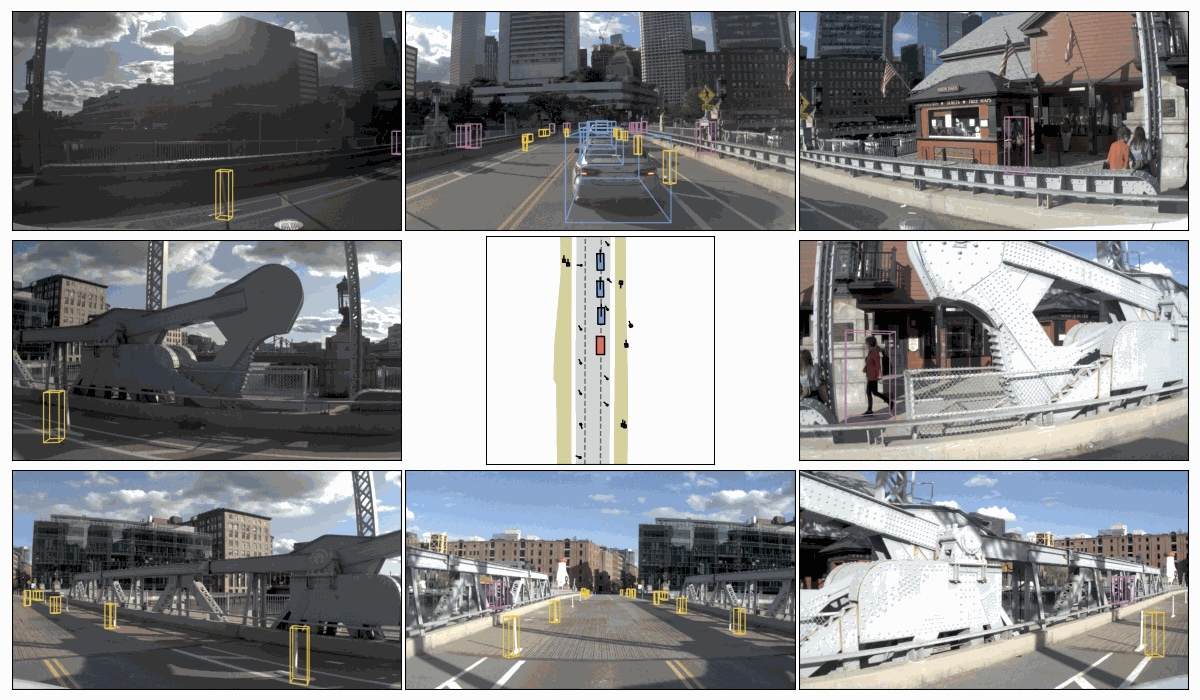
\includegraphics[width=0.8\linewidth]{images/data-sample-1.jpg}
    \hfill
    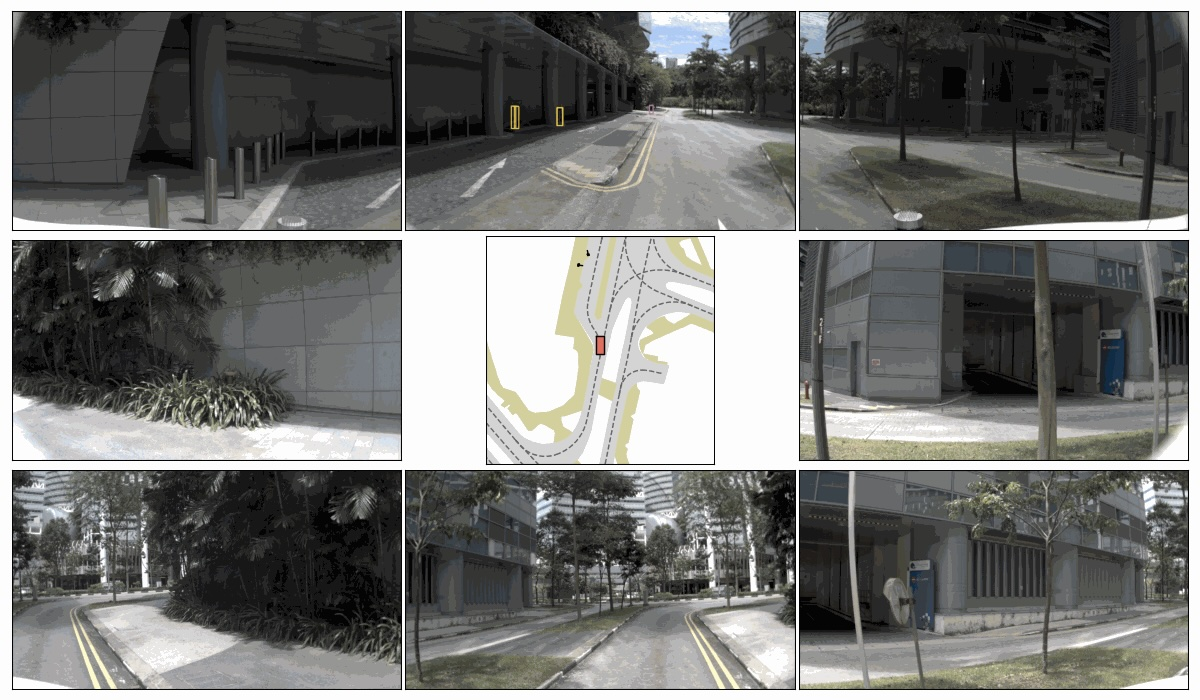
\includegraphics[width=0.8\linewidth]{images/data-sample-2.jpg}
    }
    \caption{NAVSIM frames of various cameras and sensors}
    \label{fig:navsim_scenario}
\end{figure}


\section{Approach: I-JEPA-based End-to-End Driving}
\label{sec:approach}
\begin{figure}[ht]
    \centering
    % Resize the whole picture to fit the line width
    \resizebox{\linewidth}{!}{% Add this line
    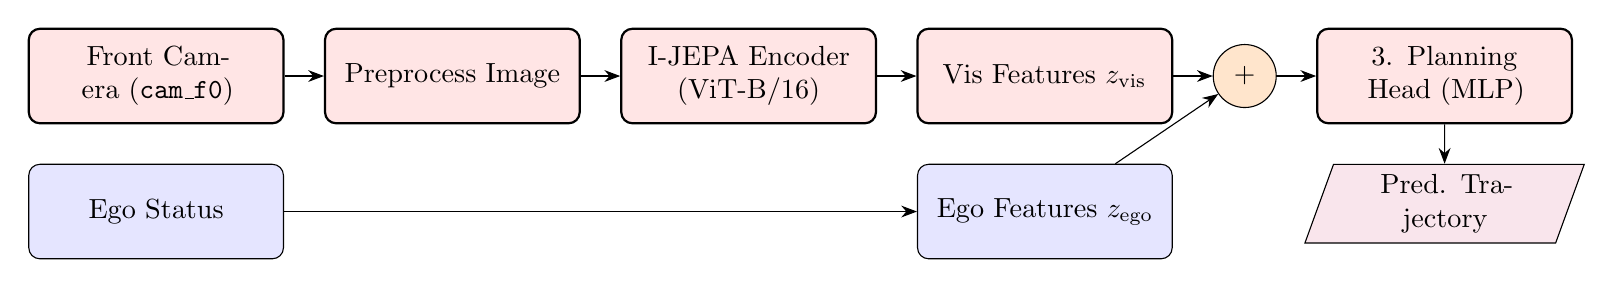
\begin{tikzpicture}[
        node distance=1cm and 1.5cm, % Keep original distances for now
        block/.style={rectangle, draw, fill=blue!10, rounded corners,
                      text width=3cm, text centered, minimum height=1.2cm},
        data/.style={ellipse, draw, fill=green!10, text centered, minimum width=2cm},
        arrow/.style={-{Stealth[length=2mm, width=1.5mm]}},
        concat/.style={circle, draw, fill=orange!20, minimum size=0.8cm, inner sep=0pt, node contents={+}},
        module/.style={rectangle, draw, fill=red!10, rounded corners, thick,
                       text width=3cm, text centered, minimum height=1.2cm},
        output/.style={trapezium, trapezium left angle=70, trapezium right angle=110, draw, fill=purple!10,
                       text width=2.5cm, text centered, minimum height=1cm},
        comment/.style={rectangle, text width=4cm, align=left, font=\small\itshape}
      ]

      % --- Original TikZ Nodes and Arrows ---
      % Input Data Nodes
      % \node (navsim) [block, fill=gray!10] {NAVSIM};
      \node (cam_img) [module] {Front Camera (\texttt{cam\_f0})}; % Shortened text
      \node (ego_status) [block, below=0.5cm of cam_img] {Ego Status}; % Shortened text

      % Processing Steps
      \node (preprocess) [module, right=0.5cm  of cam_img] {Preprocess Image}; % Shortened text
      \node (encoder) [module, right=0.5cm  of preprocess] {I-JEPA Encoder (ViT-B/16)}; % Shortened text
      \node (vis_feat) [module, right=0.5cm  of encoder] {Vis Features $z_{\text{vis}}$}; % Shortened text
      \node (ego_feat) [block, below=0.5cm  of vis_feat] {Ego Features $z_{\text{ego}}$};

      % % Fusion and Planning Head
      \node (concatenate) [concat, right=0.5cm of vis_feat] {};
      \node (head) [module, right=0.5cm of concatenate] {3. Planning Head (MLP)};
      \node (traj_pred) [output, below=0.5cm of head] {Pred. Trajectory}; % Shortened text

      % % Arrows indicating data flow
      \draw [arrow] (cam_img) -- (preprocess);
      \draw [arrow] (preprocess) -- (encoder);
      \draw [arrow] (encoder) -- (vis_feat);
      \draw [arrow] (ego_status) -- (ego_feat);
      \draw [arrow] (vis_feat) -- (concatenate);
      \draw [arrow] (ego_feat) -- (concatenate);
      \draw [arrow] (concatenate) -- (head);
      \draw [arrow] (head) -- (traj_pred);

    \end{tikzpicture}
    } % Add this closing brace for resizebox
    \caption{Pipeline for the I-JEPA-based planning agent in NAVSIM.} % Shortened caption
    \label{fig:pipeline}
\end{figure}


Figure~\ref{fig:pipeline} provides a high-level overview of our proposed system. The pipeline integrates a pre-trained I-JEPA visual encoder with a trainable planning head to enable end-to-end trajectory prediction within the NAVSIM framework. Specifically, the front camera image is first encoded into high-level semantic representations using the I-JEPA encoder, which has been pre-trained self-supervisedly. These visual features are then concatenated with the ego vehicle’s kinematic state (velocity, acceleration, and navigation command) and passed to a lightweight multilayer perceptron (MLP) that outputs the predicted future trajectory. By leveraging the general-purpose representations from I-JEPA, our approach aims to achieve label-efficient fine-tuning for the autonomous driving planning task.

% \subsection{Pre-trained I-JEPA Encoder}
% \label{subsec:encoder}
% The implementation of I-JEPA with NAVSIM will enable NAVSIM to produce new and better driving policies. This new state of the art driving policies will enable autonomous vehicles to mimic human behavior thus enabling machines to think more like humans. I-JEPA’s ability to learn from data-dense images and convert them to latent space representations without contrastive negatives or generative decoders presents a great alternative to other models such as (SimCLR, BYOL) [2, 3] and masked autoencoders (MAE) [4]. The way I-JEPA will be implemented and used in NAVSIM will be split into different stages in which the final will be the integration into NAVSIM[5]. 

% Pre-Training Options:

% Pre-Train I-JEPA on NAVSIM camera images to obtain robust ViT-based visual encoder. In order to pre-train I-JEPA there are two options available to complete this task. First would be leveraging an ImageNet pre-trained I-JEPA Vision transformer(ViT B/16) provided by Meta AI \cite{assran2023ijepa} as a partially fine-tuned feature extractor. Specifically, we adopt the \textbf{ViT-B/16} model pre-trained on ImageNet-1K. From the full I-JEPA architecture, we retain only the \textbf{context encoder} ($f_\theta$) and discard the target encoder ($f_{\bar{\theta}}$) and predictor ($g_\phi$). The ViT-B/16 architecture expects input images of size $224 \times 224$. The second option would be to download all the datasets needed from NAVSIM into local memory and pre-train I-JEPA with this data. Downloading the NAVSIM data locally requires about 2 TB of storage which would be downloaded onto a 5 TB Seagate HDD external memory card. Below will be the explanation of how both of these options would be achieved.

% Inputs: 
% Streams of past frames from onboard sensors, such as cameras, LiDAR [13]. Hence some driving agents in NAVSIM need to plan trajectory as a sequence of future poses or movements over a specific future time frame in 'x' seconds, it leverages a dataset of frames captures by it's on board sensors to facilitate this task. The data provided by NAVSIM was retrieved from the OpenScene dataset [14].  This closed loop planning is different from other real world simulation environment in a way that the data that is fed onto the planning model is only based on the initial real world sensor sample. Then any extra sensory data during a specific timeframe such as in x seconds is not added or used. This makes the planning more challenging for the agent. By using I-JEPA it is hoped to pre-train it to understand these initial sensor data and make an adequate decision over a short duration. Unlike other models I-JEPA only cares about high level unlabeled data thus reproducing how the brain works of a human being. Our brain only makes a decision while driving with the data that is fed to is through our eyesight at present time thus enabling us to make last second decisions. It is hoped that by pre-training I-JEPA with the extensive data obtained from OpenScene then it will be able to make a decision faster than other agents. This way of using non-reactive simulation in NAVISM not only will predict the next steering action, but also show other benchmarks to reflect safety, comfort and progress. These benchmarks can be used to compare this model to others.  It is also good to note that by embedding LiDAR cloud data onto camera images will help delete faulty or blurred data from low quality images this improving the data quality. 

% Process: Pre-Training with dataset
% \begin{figure}
%     \centering
%     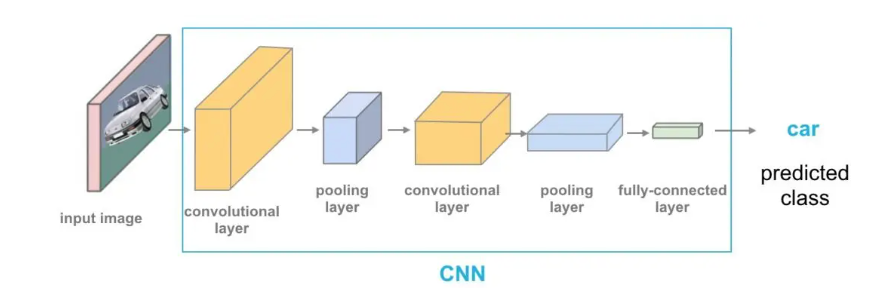
\includegraphics[width=0.5\linewidth]{project/approach/images/cnn.png}
%     \caption{Typical CNN Architecture}
%     \label{fig:enter-label}
% \end{figure}
% One of the big selling points of using I-JEPA compared to a CNN based agent would be the fact that it uses a Vision Transformer. Not only has the I-JEPA vision transformer achieved highly competitive performance in benchmark compared to other CNN based architectures but it has been tested to be faster than some. Rather than approaching each image and passing it through multiple layers. I-JEPA will obtain the real image datasets from OpenScene and depending on the scenario predict the appropriate course of action such as in our case (predicting the steering degree to take place for the vehicle). We plan on using the output from I-JEPA to create a predictor in which it will decide to stay in the lane of the road, and also to take the appropriate action in case of obstacles such as steering the wheel clockwise or counter clock wise to a certain angle to avoid collision. Using Navsim will prove to be helpful since it also provides a way to predict the time to collision which can be used to estimate the distance from an object to the EGO vehicle. The main purpose of this task would be to showcase how using I-JEPA will output good benchmark scores compared to other models, and prove to be faster at decision making. 

% Benchmarks against other models will be provided at the end of the project.  
% For each timestep within a NAVSIM scenario provided to the agent, the following steps are performed:
% \begin{enumerate}
%     \item The image from the front camera (\texttt{cam-f0}) is extracted.
%     \item The image is resized/cropped to $224 \times 224$ pixels.
%     \item Standard ImageNet normalization is applied (mean=[0.485, 0.456, 0.406], std=[0.229, 0.224, 0.225]), matching the expected input statistics of the pre-trained model.
%     \item The preprocessed image is fed into the ViT-B/16 context encoder.
%     \item The output \texttt{[CLS]} token embedding is extracted as the primary visual feature representation, $z_{\text{vis}} \in \mathbb{R}^{768}$.
% \end{enumerate}
% During fine-tuning, we explore two strategies:
% \begin{itemize}
%     \item \textbf{Stage 1 (Frozen Encoder):} All parameters of the ViT-B/16 encoder are kept frozen. Only the planning head parameters are updated.
%     \item \textbf{Stage 2 (Partial Fine-tuning, Optional):} After initial training of the head, the final few layers (e.g., the last transformer block and layer normalization) of the ViT encoder are unfrozen and fine-tuned jointly with the planning head, using a significantly reduced learning rate compared to the head.
% \end{itemize}z


\subsection{Pre-trained I-JEPA Encoder}
\label{subsec:encoder}
% State the chosen approach directly and justify it.
Our approach leverages a publicly available, pre-trained I-JEPA model to serve as the visual encoder for our NAVSIM planning agent. This strategy allows us to utilize powerful, general-purpose visual features learned on large-scale datasets (ImageNet-1K) without undertaking the computationally intensive self-supervised pre-training process ourselves. We specifically adopt the official \textbf{ViT-B/16} I-JEPA checkpoint released by Meta AI \cite{assran2023ijepa}.

% Specify which parts are used and discarded.
From the complete I-JEPA architecture associated with the checkpoint, we isolate and utilize only the \textbf{context encoder} component ($f_\theta$). The target encoder ($f_{\bar{\theta}}$) and the predictor network ($g_\phi$), which are essential for the I-JEPA pre-training objective, are discarded for our downstream planning task.

% Detail the integration process: how the encoder processes NAVSIM input.
The selected ViT-B/16 context encoder has specific input requirements. To integrate it into our NAVSIM agent, the following processing pipeline is applied at each timestep the agent needs to make a prediction:
\begin{enumerate}
    % Step 1: Input Extraction - Explicitly mention the source camera.
    \item The image from the ego-vehicle's primary front camera (\texttt{cam\_f0}) is obtained from the current NAVSIM scenario data \cite{dauner2024navsim, OpenScene2023}.
    % Step 2: Preprocessing - Must match pre-training.
    \item The extracted image undergoes preprocessing to match the conditions under which the ViT-B/16 encoder was pre-trained: it is resized and center-cropped to $224 \times 224$ pixels.
    % Step 3: Normalization - Crucial for pre-trained models.
    \item Standard ImageNet normalization statistics (mean=[0.485, 0.456, 0.406], std=[0.229, 0.224, 0.225]) are applied to the pixel values.
    % Step 4: Encoder Forward Pass - The core step.
    \item The preprocessed image tensor is then passed through the loaded ViT-B/16 context encoder ($f_\theta$).
    % Step 5: Feature Extraction - Specify the exact feature used.
    \item The final visual feature representation for the planning head is obtained by extracting the output embedding corresponding to the special \texttt{[CLS]} token \cite{dosovitskiy2020vit}. For the ViT-B/16 architecture, this results in a feature vector $z_{\text{vis}} \in \mathbb{R}^{768}$.
\end{enumerate}

% Describe how the encoder's weights are handled during downstream fine-tuning.
During the subsequent fine-tuning phase on the NAVSIM trajectory prediction task (detailed in Sec.~\ref{subsec:subset}), the parameters of this pre-trained encoder are managed according to one of two strategies:
\begin{itemize}
    \item \textbf{Stage 1 (Frozen Encoder):} Initially, all parameters of the loaded ViT-B/16 encoder are frozen (i.e., their gradients are not computed or updated). Training only affects the parameters of the planning head (Sec.~\ref{subsec:head}). This stage evaluates the direct utility of the off-the-shelf ImageNet-trained I-JEPA features for the driving task.
    \item \textbf{Stage 2 (Partial Fine-tuning, Optional):} After an initial training period with the encoder frozen, we may selectively unfreeze the parameters of the final transformer block(s) and associated layer normalization layers within the ViT encoder. These layers, along with the planning head, are then trained jointly, typically employing a much smaller learning rate for the encoder parameters ($\alpha_{\text{enc}}$) compared to the head ($\alpha_{\text{head}}$) (e.g., $\alpha_{\text{enc}} = \alpha_{\text{head}} / 10$). This allows the higher-level features of the encoder to adapt slightly to the specific visual characteristics of the NAVSIM environment while aiming to preserve the robust representations learned during pre-training.
\end{itemize}

% \subsection{Planning Head}
% \label{subsec:head}
% We employ a simple Multi-Layer Perceptron (MLP) as the planning head. This head takes the concatenated visual features and ego status information as input and predicts the future trajectory.
% \begin{itemize}
%     \item \textbf{Input Features:} The input to the MLP is the concatenation of the visual feature $z_{\text{vis}} \in \mathbb{R}^{768}$ (from the I-JEPA encoder's \texttt{[CLS]} token) and the current ego status features $z_{\text{ego}} \in \mathbb{R}^{7}$. The ego status features consist of 2D velocity, 2D acceleration, and a 3-dimensional one-hot encoding of the driving command (left, right, straight), resulting in a combined input dimension of $768 + 7 = 775$.
%     \item \textbf{Architecture:} The MLP consists of two hidden layers, each with 256 neurons and ReLU activation functions.
%     \item \textbf{Output:} The final linear layer maps the 256-dimensional hidden representation to the flattened trajectory parameters. For a 4-second horizon sampled at 0.5-second intervals ($N_{\text{poses}} = 8$), the output dimension is $N_{\text{poses}} \times 3 = 8 \times 3 = 24$. This output is then reshaped into the trajectory format $[N_{\text{poses}}, 3]$, where each row represents $(x, y, \theta)$ in the local ego-vehicle coordinate frame at future timesteps $\{0.5, 1.0, \dots, 4.0\}\,\text{s}$.
%     \item \textbf{Training Loss:} The planning head (and optionally the unfrozen encoder layers) is trained using an $L_1$ loss between the predicted trajectory and the ground-truth future trajectory recorded by the human driver in the NAVSIM logs.
% \end{itemize}

\subsection{Planning Head}
\label{subsec:head}
The planning head serves as the crucial component that maps the rich features extracted by the visual encoder and the current vehicle state into a concrete future trajectory plan. For this initial investigation, we employ a relatively simple \textbf{Multi-Layer Perceptron (MLP)} architecture for this head.

% Justification for choosing MLP
The choice of an MLP is deliberate, driven by several factors:
\begin{itemize}
    \item \textbf{Simplicity and Efficiency:} MLPs are straightforward to implement, computationally efficient to train and run, and provide a solid baseline for regression tasks.
    \item \textbf{Focus on Features:} By using a simple head, we aim to primarily evaluate the quality and utility of the semantic features ($z_{\text{vis}}$) derived from the pre-trained I-JEPA encoder. A more complex head (e.g., a Transformer decoder) might achieve higher performance but could also obscure whether improvements stem from the head's architecture or the input features themselves.
    \item \textbf{Baseline Establishment:} It establishes a performance benchmark. If strong results can be achieved even with this simple head, it strongly suggests the high quality of the I-JEPA features for this task. Future work could then explore more complex head architectures.
\end{itemize}

% Detailed Structure Description
The specific structure of our MLP planning head is as follows:
\begin{itemize}
    \item \textbf{Input Features:} The input layer receives the concatenated feature vector, combining the visual embedding $z_{\text{vis}} \in \mathbb{R}^{768}$ (from the I-JEPA encoder's \texttt{[CLS]} token, Sec.~\ref{subsec:encoder}) and the current ego status features $z_{\text{ego}} \in \mathbb{R}^{7}$ (2D velocity, 2D acceleration, and a 3-dimensional one-hot encoding for the driving command: left, right, or straight). This results in a combined input vector of dimension $768 + 7 = 775$.
    \item \textbf{Hidden Layers:} The MLP incorporates two hidden layers.
        \begin{itemize}
            \item The first hidden layer performs a linear transformation from the 775-dimensional input to 256 neurons, followed by a Rectified Linear Unit (ReLU) activation function. ReLU is chosen for its computational efficiency and ability to introduce non-linearity, allowing the network to model complex relationships.
            \item The second hidden layer applies another linear transformation from 256 neurons to 256 neurons, again followed by a ReLU activation.
        \end{itemize}
    \item \textbf{Output Layer:} A final linear layer maps the 256-dimensional representation from the last hidden layer to the required output dimension for the trajectory. For the standard NAVSIM 4-second planning horizon sampled at 0.5-second intervals ($N_{\text{poses}} = 8$), the output consists of 8 poses, each with $(x, y, \theta)$ coordinates. Therefore, the output layer has $N_{\text{poses}} \times 3 = 8 \times 3 = 24$ neurons. This layer uses \textit{no activation function}, as is standard for regression tasks where the output values are unbounded (or bounded by subsequent processing/interpretation rather than the activation itself).
    \item \textbf{Output Reshaping:} The flattened 24-dimensional output vector is then reshaped into the standard trajectory format $[N_{\text{poses}}, 3]$ (i.e., $[8, 3]$), where each row represents the predicted $(x, y, \theta)$ pose in the local ego-vehicle coordinate frame at future timesteps $\{0.5, 1.0, \dots, 4.0\}\,\text{s}$.
\end{itemize}

% Justification for L1 Loss
\paragraph{Training Loss:}
The parameters of the planning head (and potentially the unfrozen encoder layers during Stage 2 fine-tuning) are optimized by minimizing the \textbf{L1 loss} (Mean Absolute Error) between the predicted trajectory and the ground-truth future trajectory recorded by the human driver in the NAVSIM logs.

L1 loss was chosen over alternatives like L2 loss (Mean Squared Error) for several reasons relevant to trajectory regression:
\begin{itemize}
    \item \textbf{Robustness to Outliers:} L1 loss is generally less sensitive to large errors or outliers in the ground-truth data compared to L2 loss, which squares the difference. Human driving trajectories can occasionally contain sharp, atypical maneuvers which might unduly influence a model trained with L2 loss.
    \item \textbf{Direct Interpretation:} L1 loss directly minimizes the average absolute error in predicted coordinates and heading, providing an interpretable penalty on the magnitude of deviation from the ground truth.
    \item \textbf{Common Practice:} L1 loss is frequently employed for trajectory prediction tasks in autonomous driving literature, facilitating comparisons and aligning with established practices.
\end{itemize}

\subsection{Fine-tuning on NAVSIM Subsets}
\label{subsec:subset}
The standard training configuration within the NAVSIM framework utilizes the \texttt{navtrain} split \cite{dauner2024navsim}. This split is itself a curated filter applied to the large OpenScene \texttt{trainval} dataset logs, specifically selecting over 100,000 challenging driving scenarios where simple heuristic policies often fail. While NAVSIM offers optimized sensor data downloads for \texttt{navtrain} (approx. 445GB), processing even this curated split for numerous experiments can be demanding under the NYU HPC quota limitations and time constraints.

Therefore, to ensure feasible training times and resource usage, our fine-tuning experiments are conducted on a further \textbf{randomly selected subset} derived from the official \texttt{navtrain} split. We define a fixed subset fraction, specifically \textbf{10\%} (corresponding to \(\approx\) 10,300 scenarios), sampled once based on scenario tokens. This fixed training subset is used consistently across all experiments, including the training of baseline models (Sec.~\ref{sec:experiments}) and the label efficiency analysis, ensuring fair comparisons.

From this selected training subset, a small portion (e.g., 10\%) is held out to form a distinct \textbf{validation subset}. This validation set is used exclusively for monitoring training progress (e.g., validation loss) and potentially for early stopping, preventing overfitting to the training subset. The NAVSIM \texttt{Dataset} class and data loading scripts are configured to load only the scenario tokens corresponding to our defined training and validation subsets.

The fine-tuning process will make use the AdamW optimizer \cite{loshchilov2017decoupled} with default hyperparameters, except for the learning rate. We train for a maximum of 50 epochs, using the validation subset loss for potential early stopping. A base learning rate, $\alpha_{\text{head}}$, is applied to the parameters of the planning head (Sec.~\ref{subsec:head}). 

For the Stage 2 partial fine-tuning (Sec.~\ref{subsec:encoder}), the learning rate for the unfrozen encoder parameters, $\alpha_{\text{enc}}$, is reduced, $\alpha_{\text{enc}} = \alpha_{\text{head}} / 10$. To gauge the robustness of our findings concerning the chosen subset and training stochasticity, key experiments may be repeated using multiple random seeds for the initial subset sampling and model weight initialization.

\section{Experiments in NAVSIM}
\label{sec:experiments}
We outline a series of experiments designed to rigorously evaluate the performance and data efficiency of the proposed \texttt{IJEPAPlanningAgent} within the NAVSIM environment \cite{dauner2024navsim}.

\paragraph{Experimental Setup.}
All training and evaluation procedures will adhere to the NAVSIM framework standards. Fine-tuning will be performed using the training subset derived from \texttt{navtrain}, as detailed in Sec.~\ref{subsec:subset}. Final performance evaluation will ideally utilize the official \texttt{navtest} split. However, acknowledging potential HPC resource constraints associated with metric caching and evaluation on the full \texttt{navtest} set, we may need to perform final evaluations on a consistently sampled test subset (e.g., matching the proportion of the training subset relative to \texttt{navtrain}). The specific test set configuration used (full \texttt{navtest} or a defined subset) will be clearly documented. Metric caching will be performed using the \texttt{run\_metric\_caching.py} script, and evaluations will be executed using \texttt{run\_pdm\_score.py} from the NAVSIM toolkit. The primary performance metric is the overall PDM-Score, supplemented by analysis of key sub-metrics (NC, DAC, EP, TTC, C) to understand specific behavioral aspects.

\paragraph{Baseline Methods.}
To contextualize the performance of our I-JEPA-based agent, we will compare it against established NAVSIM baselines:
\begin{enumerate}
    \item \textbf{Constant Velocity Agent:} A deterministic, non-learning baseline provided by NAVSIM, serving as a lower bound indicating performance achievable without learning or environment perception. It extrapolates motion based on the initial velocity.
    \item \textbf{Ego Status MLP Agent:} A learning-based baseline utilizing an MLP architecture identical to our planning head (Sec.~\ref{subsec:head}), but receiving only ego status features ($z_{\text{ego}}$) as input. Crucially, this agent will be trained using the \textit{exact same training subset, optimization strategy, and number of epochs} as the \texttt{IJEPAPlanningAgent}'s planning head. This ensures a direct comparison to isolate the contribution of the I-JEPA visual features.
    \item \textbf{(Optional) Transfuser Agent \cite{chitta2023transfuser}:} If readily available pre-trained weights for NAVSIM exist and evaluation is feasible, we may include Transfuser as a state-of-the-art reference. This comparison would acknowledge Transfuser's architectural complexity and its use of multi-modal inputs (including LiDAR), contrasting it with our vision-only approach.
\end{enumerate}

\paragraph{Main Performance Comparison.}
The core evaluation involves comparing the best PDM-Score achieved by the \texttt{IJEPAPlanningAgent} against the baseline methods on the designated test set (or subset). We will evaluate the performance after Stage 1 fine-tuning (frozen encoder) and, if pursued, after Stage 2 (partial fine-tuning) to assess the impact of adapting the encoder features. This comparison aims to quantify the absolute performance gain achieved by incorporating I-JEPA visual features over simpler approaches.

\paragraph{Label Efficiency Analysis.}
A key hypothesis is that I-JEPA pre-training enhances data efficiency. To investigate this, we will conduct an ablation study focused on the amount of labeled data used during fine-tuning. We will train multiple instances of both the \texttt{IJEPAPlanningAgent} (in its Stage 1 configuration with a frozen encoder) and the \texttt{EgoStatusMLPAgent}. Each training run will utilize a different fraction of our selected \textit{training subset} – for example, using scenarios corresponding to {1\%, 5\%, 10\%, 50\%, 100\%} of the tokens within our [10\%] \texttt{navtrain} subset. Following training, each resulting model will be evaluated on the \textit{same fixed test set (or subset)}. The results will be presented by plotting the final PDM-Score achieved versus the percentage of the training subset used. We expect the \texttt{IJEPAPlanningAgent} to exhibit a slower degradation in performance as the training data fraction decreases compared to the \texttt{EgoStatusMLPAgent}, thereby demonstrating superior label efficiency attributable to the pre-trained features.

% \begin{figure}[h]
%     \centering
%     % Placeholder: Replace with your actual plot later
%     \includegraphics[width=0.6\linewidth]{placeholder_label_efficiency.png}
%     \caption{Planned evaluation: PDM-Score vs. fraction of labeled training subset. We expect the I-JEPA agent (blue) to outperform the Ego Status MLP baseline (orange), especially in the low-data regime.}
%     \label{fig:efficiency_plan}
% \end{figure}

\section{Discussion and Conclusion}
\label{sec:conclusion}

\paragraph{Discussion.}
This work proposed and detailed a methodology for integrating pre-trained I-JEPA visual representations into an end-to-end trajectory planning agent for the NAVSIM benchmark. By leveraging readily available, powerful self-supervised models, we aim to bypass the need for extensive task-specific pre-training or complex multi-modal architectures commonly employed in autonomous driving research. The core of our approach involves using an ImageNet-trained ViT-B/16 I-JEPA context encoder as a feature extractor, combined with a simple MLP planning head fine-tuned on NAVSIM data subsets.

The success of this approach, evaluated through the experiments outlined in Sec.~\ref{sec:experiments}, would provide valuable insights. Achieving competitive PDM-Scores compared to the Ego Status MLP baseline would validate the utility of the transferred I-JEPA features for the planning task. Furthermore, demonstrating superior performance in the low-data regime during the label efficiency analysis would strongly support the hypothesis that SSL pre-training, specifically I-JEPA's approach focused on semantic representation, can significantly reduce the reliance on large labeled datasets for training competent driving policies. This has implications for accelerating the development cycle and reducing the cost associated with autonomous vehicle software development.

However, it is crucial to acknowledge the inherent limitations of this study. Firstly, the \textbf{domain gap} between ImageNet (where the I-JEPA encoder was pre-trained) and the NAVSIM driving environment (urban scenes, specific camera characteristics) may limit feature transferability. While fine-tuning (Stage 2) might mitigate this partially, the features might not be perfectly optimal for driving-specific nuances. Secondly, our reliance on \textbf{data subsets} for fine-tuning and potentially evaluation, necessitated by HPC constraints, means that the absolute performance metrics reported might not be directly comparable to results obtained on the full \texttt{navtrain} and \texttt{navtest} splits. The conclusions drawn will be relative to the performance achievable \textbf{within} these subsets. Thirdly, the proposed agent is \textbf{vision-only}. It deliberately omits LiDAR and detailed HD map information, which are known to be beneficial for robust planning \cite{chitta2023transfuser}. This limits the agent's potential performance compared to state-of-the-art multi-modal systems but allows for a focused analysis of the contribution of the pre-trained visual features. Lastly, the chosen \textbf{MLP planning head} is intentionally simple; more complex architectures (e.g., Transformers, RNNs) might be capable of better utilizing the rich features from the I-JEPA encoder, potentially unlocking higher performance.

\paragraph{Future Work.}
Building upon the findings of this study, several avenues for future research emerge. Investigating I-JEPA models pre-trained on large-scale, unlabeled driving datasets (rather than ImageNet) could significantly reduce the domain gap. Exploring more sophisticated planning head architectures capable of temporal reasoning or attention mechanisms might better leverage the ViT features. Developing methods to effectively fuse the I-JEPA visual features with other modalities like LiDAR point clouds or structured map representations within the NAVSIM framework presents another promising direction. Finally, if resources permit, repeating the fine-tuning and evaluation on the complete \texttt{navtrain} and \texttt{navtest} splits would provide definitive benchmarks.

\paragraph{Conclusion.}
This paper presents a feasible and structured approach for investigating the application of I-JEPA, a powerful self-supervised learning technique, to the task of end-to-end trajectory planning in the NAVSIM simulator. By utilizing pre-trained models and adapting the fine-tuning process for realistic resource constraints via data subsetting, we aim to evaluate the effectiveness and, crucially, the label efficiency benefits offered by I-JEPA's semantic visual representations. If successful, this work will contribute valuable evidence supporting the use of large-scale SSL models as effective off-the-shelf components for building more data-efficient and capable autonomous driving systems.

% \section*{Acknowledgments}
% We thank the NYU HPC facility for providing computational resources. We also acknowledge the developers of NAVSIM \cite{dauner2024navsim} and the contributors to the OpenScene dataset \cite{OpenScene2023} for making their resources publicly available. We thank Meta AI for releasing the pre-trained I-JEPA models \cite{assran2023ijepa}. This work was supported by the Department of Electrical and Computer Engineering at NYU Tandon School of Engineering.

% --- Bibliography ---
\newpage
\bibliographystyle{unsrt} % Simple numeric style like [1], [2], ...
\bibliography{references}
\end{document}